\documentclass[11pt,A4]{article}
\usepackage[T1]{fontenc}
\usepackage[utf8]{inputenc}
\usepackage[UKenglish]{babel}
\usepackage{mathtools}
\usepackage{amsthm}
\usepackage{amssymb}
\usepackage{manfnt}
\usepackage{marginnote}
\usepackage[dvipsnames]{xcolor}
%\usepackage{mathrsfs}
\usepackage[mathscr]{euscript}
\usepackage{enumitem}
\usepackage{tikz-cd}
\usepackage{hyperref}
\usepackage[noabbrev]{cleveref}
\usepackage{todonotes}
\usepackage{bbm}
\usepackage{caption}
\usepackage{subcaption}

% Plain theorems
\theoremstyle{plain}
\newtheorem{thm}{Theorem}[section]
\newtheorem{lm}[thm]{Lemma}
\newtheorem{prop}[thm]{Proposition}
\newtheorem{cor}[thm]{Corollary}

% Definition theorems
\theoremstyle{definition}
\newtheorem{defn}[thm]{Definition}
\newtheorem{nota}[thm]{Notation}
\newtheorem{exa}[thm]{Example}
\newtheorem{pbl}[thm]{Problem}
\newtheorem{q}[thm]{Question}

% Remark theorems
\theoremstyle{remark}
\newtheorem{rem}[thm]{Remark}
\newtheorem{exe}[thm]{Exercise}

% Mathbb
\newcommand{\N}{\mathbb{N}}
\newcommand{\Z}{\mathbb{Z}}
\newcommand{\Q}{\mathbb{Q}}
\newcommand{\R}{\mathbb{R}}
\newcommand{\1}{\mathbbm{1}}
\newcommand{\C}{\mathbb{C}}
\renewcommand{\P}{\mathbb{P}}
\newcommand{\CP}{\mathbb{CP}}
\newcommand{\bbE}{\mathbb{E}}
\newcommand{\bbD}{\mathbb{D}}
\newcommand{\cbbD}{\bar{\mathbb{D}}}

% Mathscr for categories
\newcommand{\scrC}{\mathscr{C}}
\newcommand{\Top}{\mathscr{T}op}
\newcommand{\CHaus}{\mathscr{CH}aus}
\newcommand{\ED}{\mathscr{ED}}
\newcommand{\A}{\mathscr{A}}
\newcommand{\CG}{\mathscr{CG}}
\newcommand{\Ab}{\mathscr{A}b}
\newcommand{\Set}{\mathscr{S}et}
\newcommand{\D}{\mathscr{D}}
\newcommand{\K}{\mathscr{K}}
\newcommand{\Db}{\mathscr{D}^{\mathrm{b}}}
\newcommand{\QCoh}{\mathscr{QC}oh}
\newcommand{\Coh}{\mathscr{C}oh}

% Mathcal for sheaves
\newcommand{\calC}{\mathcal{C}}
\newcommand{\F}{\mathcal{F}}
\newcommand{\G}{\mathcal{G}}
\renewcommand{\L}{\mathcal{L}}
\newcommand{\M}{\mathcal{M}}
\renewcommand{\O}{\mathcal{O}}
\newcommand{\U}{\mathcal{U}}
\newcommand{\X}{\mathcal{X}}

% Math operators
\DeclareMathOperator{\Hom}{Hom}
\DeclareMathOperator{\Ext}{Ext}
\DeclareMathOperator{\Fun}{Fun}
\DeclareMathOperator{\Cond}{Cond}
\DeclareMathOperator{\Ob}{Ob}
\DeclareMathOperator{\im}{im}
\DeclareMathOperator{\coker}{coker}
\DeclareMathOperator{\PSh}{PSh}
\DeclareMathOperator{\Sh}{Sh}
\let\Re\relax
\DeclareMathOperator{\Re}{Re}
\let\Im\relax
\DeclareMathOperator{\Im}{Im}

% New commands
\newcommand{\pe}{*_{pro\acute et}}
\renewcommand{\u}[1]{\underline{#1}}
\newcommand{\ot}{\otimes}
\newcommand{\op}{\oplus}
\newcommand{\fp}[1]{\times_{#1}}
\newcommand{\id}{\mathrm{id}}
\newcommand{\ev}{\mathrm{ev}}
\newcommand{\grd}{^{\bullet}}
\newcommand{\db}{\marginnote{\dbend}}
\newcommand{\tms}{\times}
\newcommand{\sub}{\subseteq}
\newcommand{\epi}{\twoheadrightarrow}
\newcommand{\mono}{\hookrightarrow}


\title{Various lecture notes}
\author{Pedro Núñez}
\date{\today}

\begin{document}

\maketitle

\tableofcontents

\section{About these notes}

The purpose of these notes is to keep the material seen in lectures a bit organized and easily accesible from one single place, but they don't intend to be complete and they will surely be full of typos and mistakes\footnote{If you find any, please let me know! You can do this from GitHub or write me an email directly at pedro.nunez[at]math.uni-freiburg.de.}.

If interesting questions occur during the lectures they will be reflected here in \textcolor{blue}{blue color}.
If I want to add anything which was not said in the lecture, I will use \textcolor{ForestGreen}{green color} instead.

Warnings will be marked with a \href{https://en.wikipedia.org/wiki/Bourbaki_dangerous_bend_symbol}{dangerous bend} symbol on the margin \db.

\section{[CM] Talk 1 (Johan Commelin): Condensed Sets - 21.10.19}

\subsection{Introduction}

One of the main motivations for condensed mathematics is that topological algebraic objects have usually poor categorical and functorial properties.
For instance, topological abelian groups do not form an abelian category:

\begin{exa}
    $\R_{disc}\to \R$ is epi and mono, but not iso.
\end{exa}

Another motivation is coherent duality:

\begin{thm}
    Let $f\colon X\to Y$ be a proper or quasi-projective morphism of Noetherian schemes of finite Krull dimension. Then there exists a right adjoint $f^{!}$ to the derived direct image functor $f_{!}=Rf_{*}\colon \Db(\QCoh(X))\to \Db(\QCoh(Y))$.
\end{thm}

At some point analytic rings will come up.
We will then look at the category of solid modules, in which the 6-functor formalism works nicer than in the classical setting (e.g. when $f_{!}$ is not defined in the classical setting, $f_{!}$ takes non-discrete values in the condensed settings, which are "not there" in the classical setting).

\begin{defn}
    Pro\'{e}tale site of a point, denoted $\pe$, is the category of profinite sets with finite jointly surjective families of continuous maps as covers.
    A \textit{condensed set} (resp. group, ring, ...) is a sheaf of sets (resp. groups, rings, ...) on $\pe$.
    We denote by $\Cond(\scrC)$ the category of condensed objects of a category $\scrC$.
\end{defn}

\begin{defn}
    A \textit{condensed set} (resp. group, ring, ...) is a contravariant functor $X$ from $\pe$ to the category of sets (resp. groups, rings, ...) such that 
    \begin{enumerate}[label=\roman*)]
	\item $X(\varnothing)=*$.
	\item For all profinite sets $S_{1}$ and $S_{2}$ the natural map
	    \[ X(S_{1}\sqcup S_{2})\to X(S_{1})\times X(S_{2}) \]
	    is an isomorphism.
	\item For any surjection of profinite sets $f\colon S'\twoheadrightarrow S$ we get an induced\footnote{Since the pullback diagram is commutative, the image of $X(f)$ is indeed induces a morphism as claimed.} isomorphism
	    \[ X(S)\to \{ x\in X(S')\mid \pi_{1}^{*}(x)=\pi_{2}^{*}(x)\in X(S'\fp{S}S')\} \]
    \end{enumerate}
\end{defn}

We will call $X(*)$ the \textit{underlying object} in $\scrC$ of a condensed object.

\begin{rem}
    We will use $T$ for topological spaces vs. $X,Y$ for condensed sets, as opposed to Scholze's mixing of those notations.
\end{rem}

\subsection{Recollections on sheaves on sites}

Let $F$ be a presheaf on a site, which is just a contravariant functor to whatever category in which our sheaves are gonna take values.
If $U=\cup_{i}U_{i}$ is an open cover, the topological sheaf axiom could be phrased as: $F(U)$ is an equalizer of the diagram
\[ \prod_{i}F(u_{i})\rightrightarrows \prod_{i,j}F(U_{i}\cap U_{j}). \]
Note that $U_{i}\cap U_{j}$ is just the fiber product of the two inclusions.

\begin{defn}[Coverage]
    See definition 2.1 in \href{https://ncatlab.org/nlab/show/coverage}{nCat}.
\end{defn}

\begin{defn}
    $F$ a presheaf on $\scrC$.
    A collection $(s_{i})\in \prod_{i}F(U_{i})$ for $\{f_{i}\colon U_{i}\to U\}$ a covering is called a \textit{matching family} if for all $h\colon V\to U$ we have $g^{*}(s_{i})=h^{*}(s_{j})$ for $g$ and $h$ in the diagram
    \begin{center}
	\begin{tikzcd}
	    V\arrow{r}{h}\arrow{d}{g} & U_{j}\arrow{d}{f_{j}} \\
	    U_{i}\arrow{r}{f_{i}} & U
	\end{tikzcd}
    \end{center}
\end{defn}

\begin{defn}
    $F$ is a sheaf with respect to $\{U_{i}\to U\}$ if for all matching families $(s_{i})$ there exists a unique $s\in F(U)$ such that $f_{i}^{*}(s)=s_{i}$.
    We say that $F$ is a \textit{sheaf} if it is a sheaf for all covering families.
\end{defn}

\begin{rem}
    A sheaf of abelian groups is just a commutative group object in the category of sheaves of sets.
\end{rem}

\begin{thm}
    If $\scrC$ is a site, then $\Ab(\scrC)$ is an abelian category.
\end{thm}

\begin{defn}
    An additive category is a category in which the hom-sets are endowed with an abelian group structure in a way that makes composition bilinear and such that finite biproducts exist.
\end{defn}

Recall Grothendieck's axioms:
AB1) Every morphism has a kernel and a cokernel.
AB2) For every $f\colon A\to B$, the natural map $\operatorname{coim}(f)\to \im{f}$ is an iso.
AB3) All colimit exist.
AB4) AB3) + arbitrary direct sums are exact.
AB5) AB3) + arbitrary filtered colimits are exact.
AB6) AB3) + $J$ an index set, $\forall j\in J$ a filtered category (think of directed set) $I_{j}$, functors $M\colon I_{j}\to \scrC$, then
\[\varinjlim_{(i_{j}\in I_{j})_{j}}\prod_{j} M_{i_{j}}\to \prod_{j\in J}\varinjlim_{i_{j}\in I_{j}} M_{i_{j}} \]

\begin{thm}
    $\scrC$ a site. Then $\Ab(\scrC)$ satisfies AB3), AB4), AB5) and AB6).
\end{thm}

In fact, our case is even nicer:

\begin{thm}
    $\Cond(\Ab)$ in addition satisfies AB6) and AB4*).
\end{thm}

\subsection{Compactly generated topological spaces}

\begin{defn}
    A topological space $T$ is called \textit{compactly generated} if any function $f\colon T\to T'$ is continuous as soon as the composite $S\to T\to T'$ is continuous for all maps $S\to T$ where $S$ is compact and Hausdorff.
    See also \href{https://ncatlab.org/nlab/show/compactly+generated+topological+space}{nCat}.
\end{defn}

The inclusion functor $\CG \hookrightarrow \Top$ has a right adjoint $(-)^{cg}$.
If $T$ is any topological space, then the topology on $T^{cg}$ is the finest topology on $T$ such that $\sqcup_{S\to T}S\to T$ is continuous, where $S$ ranges over all compact Hausdorff spaces.

Let $T$ be a topological space.
We view $T$ as a presheaf on $\pe$ by setting $T(S)=\Hom_{\Top}(S,T)$ for all profinite sets $S$.
We denote this by $\u{T}$.
Claim: $\u{T}$ is a sheaf.
\begin{enumerate}[label=\roman*)]
    \item The first condition $\u{T}(\varnothing)=*$ is true, because there is exactly one morphism from the empty set to any topological space.
    \item $\u{T}(S_{1}\sqcup S_{2})=\u{T}(S_{1})\times \u{T}(S_{2})$ by universal property of disjoint union.
    \item For any surjection $S'\twoheadrightarrow S$ we get an isomorphism
	\[ \u{T}(S)\to \{ x\in \u{T}(S')\mid \pi_{1}^{*}(x)=\pi_{2}^{*}(x)\in \u{T}(S'\fp{S}S')\}\]
\end{enumerate}

Since $\Top\to \Cond(\Set)$ preserves products, group objects are preserved, so it maps topological groups to condensed groups etc.

\begin{prop}
    \begin{enumerate}[label=\roman*)]
	\item This functor is faithful and fully faithful when restricted to the full subcategory of compactly generated spaces.
	\item It admits a left adjoint $X\mapsto X(*)_{top}$ where $X(*)_{top}$ gets the quotient topology of $\sqcup_{S\to X}S\to X(*)$ as above.
	    The counit $I(*)_{top}\to T$ agrees with $T^{cg}\to T$.
    \end{enumerate}
\end{prop}

Coming back to our original example:

\begin{exa}
    $\mathbb{R}_{disc}\to \mathbb{R}$ can be seen in the condensed world as $\u{\mathbb{R}_{disc}}\to \u{\mathbb{R}}$, i.e. from locally constant functions to continuous functions.
    This is still a mono, but now it is not an epi.
    The cokernel $Q$ can be described as $Q(S)=\{ S\to \mathbb{R}\text{ continuous }\}/\{ S\to \mathbb{R}\text{ locally constant }\}$.
    Note in particular that the underlying set of $Q$ is just $*$, reflecting the fact that the cokernel was trivial in the classical setting.
\end{exa}

\section{[LT] Lecture 1 - 22.10.19}

\subsection{Introduction and overview of the course}

An \textit{algebraic variety} is the solution set of a family of polynomial equations in $\C^{n}$.
For example, if $f(x,y,z,t)=xy-tz$, then
\[ V(f)=\{(x,y,z,t)\in \C^{4}\mid xy-tz=0\} \]
is an algebraic variety in $\C^{4}$.
Another example would be the parabola $\{ y-x^{2}=0\}\subseteq \C^{2}$.

Let us focus on $V(f)$ and set $t=1$.
Then $X=V(f)\cap \{ t=1 \}=\{(x,y,z)\in \C^{3}\mid xy=z\}$ can be seen as a family of complex curves parametrized by the variable $z$.
For $z=0$, the complex curve $X_{0}$ has an \textit{ordinary double point} at the origin:

\begin{figure}[h]
    \centering
    \includegraphics[scale=.5]{odpfiber}
    \caption{Topological picture of our ODP.}
    \label{fig:odpfibre}
\end{figure}

Singularities arise naturally while studying the topology of algebraic varieties, and ODP's are a particularly nice kind of singularities.

For $z\neq 0$ we get an equation which looks like $xy=1$.
In this case we have the following picture:

\begin{figure}[h]
    \centering
    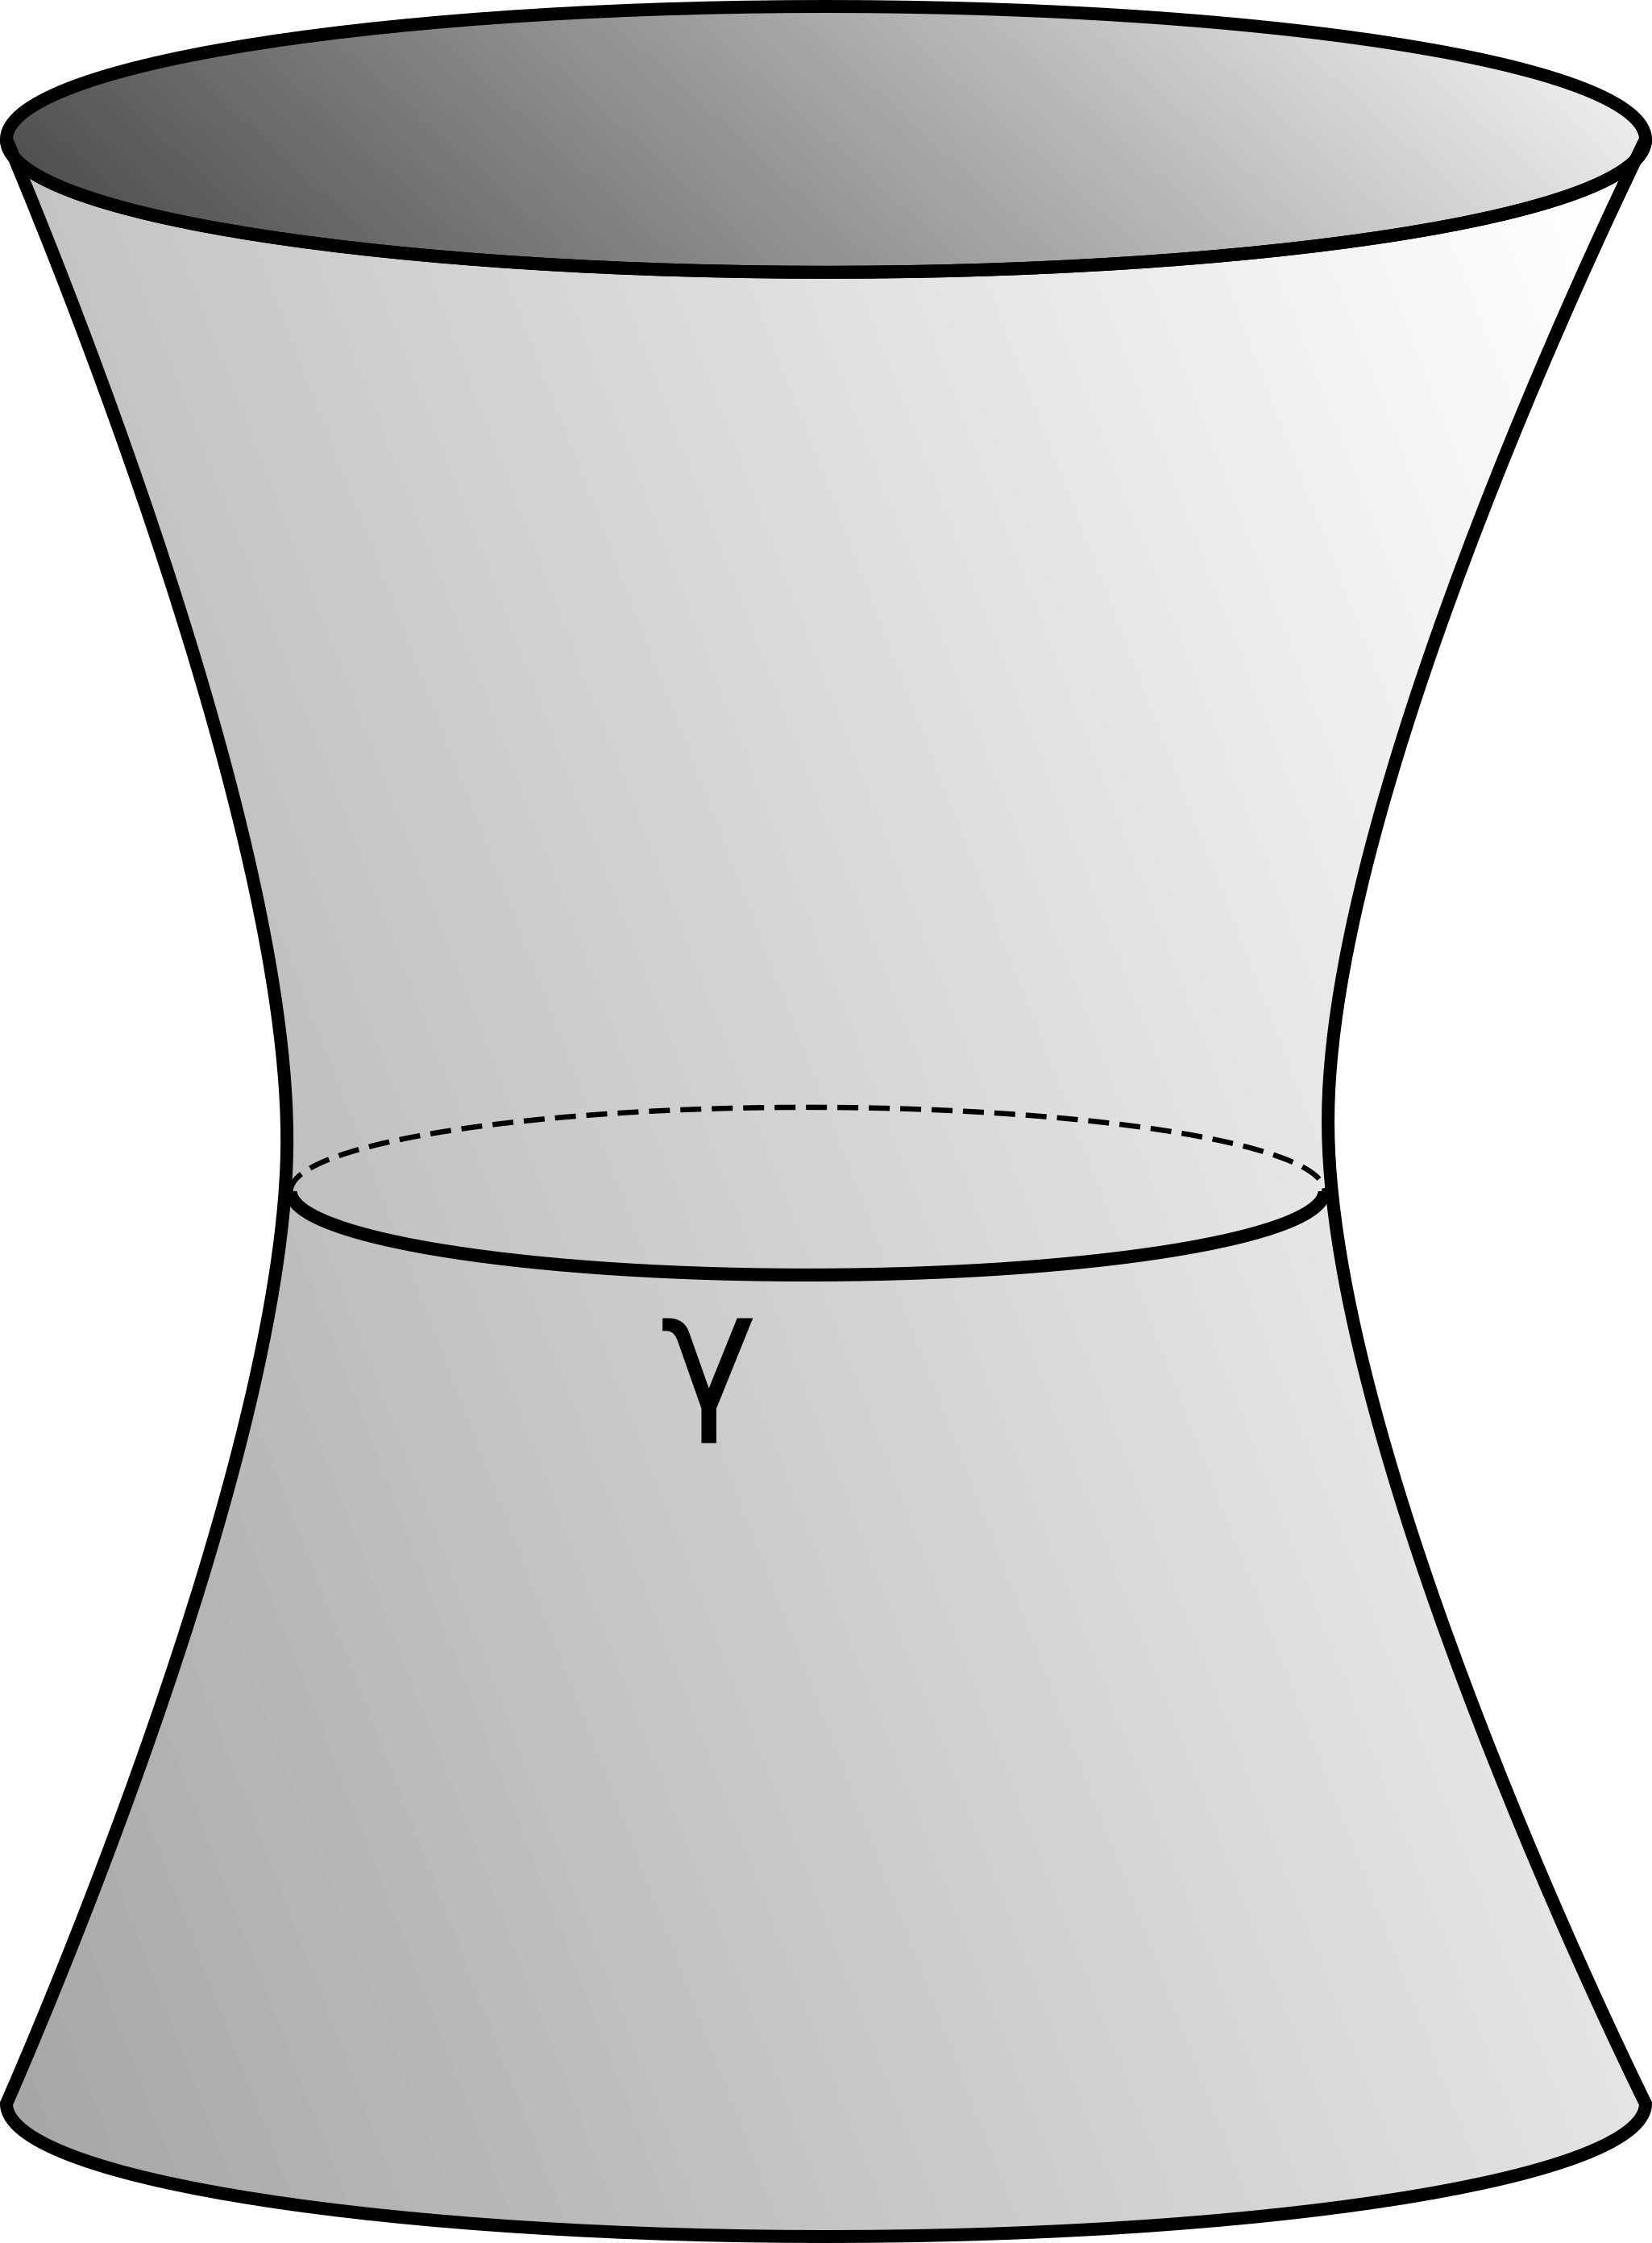
\includegraphics[scale=.8]{smoothfiber}
    \caption{Topological picture of $X_{z}$.}
    \label{fig:smoothfibre}
\end{figure}

As $z\to 0$, the central loop $\gamma$ contracts to the ordinary double point.
Note in particular that $X_{0}$ has trivial fundamental group (hence trivial $1$-homology), whereas $X_{z}$ does not.

We have a projection $\pi\colon X\to \C$, and Ehresmann's lemma tells us that for all disks $D\subseteq \C$ not containing $0$ we have $\pi^{-1}(D)\cong D\times X_{z_{0}}$ for any $z_{0}\in D$.

\begin{q}
    Given an arbitrary nonsingular algebraic variety $X\subseteq \C^{n}$, can we find a map $\pi\colon X\to \C$ such that the fibers $X_{t}$ are nonsingular for all but finitely many $t\in \C$ and such that the singular fibres have at worst ODP singularities?
\end{q}

Notice how we are missing information at infinity, e.g. $y=x^{2}$ versus $xy=1$.
The solution is to this is to replace $\C^{n}$ by $\CP^{n}$.

So let $X\subseteq\mathbb{P}^{n}$ be a nonsingular projective variety.
Then we have:

\begin{thm}
    There exists a family $(H_{t})_{t\in \CP^{1}}$ of hyperplanes in $\CP^{n}$ with $H_{[a,b]}=aH_{0}+bH_{\infty}$ such that
    \begin{enumerate}
	\item $X\subseteq \bigcup_{t\in \CP^{1}}H_{t}$.
	\item $X_{t}=X\cap H_{t}$ is nonsingular except for finitely many critical values of $t$.
	\item $X_{t}$ has ODP singularities for each critical value $t$.
    \end{enumerate}
\end{thm}

We call $(X_{t})_{t\in \CP^{1}}$ a \textit{Lefschetz pencil}.
We get a rational map $X\dashrightarrow \CP^{1}$ sending $x\mapsto t$ whenever $x\in X_{t}$.
If $x\in X_{t}\cap X_{t'}$ for $t\neq t'$, then $x\in H_{0}\cap H_{\infty}$, so this rational map is not well-defined along $X\cap H_{0}\cap H_{\infty}$.
Blowing-up this subvariety of $X$ we resolve the indeterminacy of the rational map and get a morphism $\tilde{X}\xrightarrow{\pi} \CP^{1}$ as we wanted.

As an application we obtain:

\begin{thm}[Lefschetz Hyperplane theorem]
    $X\subseteq Y\subseteq \CP^{N}$ nonsingular varieties with $X$ a hypersurface in the $n$-dimensional variety $Y$, then
    \[ H_{*}(X)\to H_{*}(Y) \]
    is an isomorphism for $*<n-1$ and a surjection for $*=n-1$.
\end{thm}

In particular, if $Y=\CP^{n}$, we have
\[ H_{*}(\CP^{n})=\begin{cases} \Z & \text{if } $*$ \text{ is even,} \\ 0 & \text{ otherwise.} \end{cases}\]
If $X\subseteq \CP^{n}$ is a nonsingular hypersurface, then its homology will be that of projective sapce on all degrees other than $n-1$.
Its $n-1$ homology will depend on the variety, e.g. the ODP (trivial $1$-homology) vs the ruled surface (with $\gamma$ non trivial on $1$-homology) from before.

\begin{exa}
    $X$ elliptic curve in $\CP^{2}$ given by $y^{2}=x(x-1)(x-\lambda)$ for $\lambda\neq 0$.
    Let $L=\CP^{1}\subseteq \CP^{2}$ and $P\in \CP^{1}\setminus (X\cup L)$.
    We get $X\xrightarrow{\pi}\CP^{1}$ by projecting from $P$ to $L$.
\end{exa}

\section{[WS] Kodaria 1 (Jin Li) - 23.10.19}

\subsection{Chow's theorem}

Let $G_{i}=G_{i}(z_{1},\ldots,z_{n})$ be homogeneous polynomials of degree $d_{i}$ for $i\in \{1,\ldots,k\}$.
Let $V=V(G_{1},\ldots,G_{k})=\{w\in \C^{n+1}\setminus \{0 \}\mid G_{i}(w)=0 \text{ for all }i\in \{1,\ldots,k\}\}\subseteq \CP^{n}$.
Assume $(\frac{\partial G_{i}}{\partial z_{j}}(w))_{i,j}$ is surjective at any $w\in V$.
By Euler's theorem on homogeneous functions we have
\[ \sum_{j=0}^{n}z_{j}\frac{\partial G_{i}}{\partial z_{j}}=d_{i}G_{i}(z_{0},\ldots,z_{n}). \]
If $\tilde{w}=(\tilde{z}_{0},\ldots,\tilde{z}_{n})\in V$, then
\[ \sum_{j=0}^{n}\tilde{z}_{j}\frac{\partial G_{i}}{\partial z_{j}}|_{\tilde{w}}=0\]
$V\cap U_{i}$ for any $i\in \{0,\ldots,n\}$, $U_{i}=\{[z_{0}:\ldots:z_{n}]\in \CP^{n}\mid z_{i}\neq 0\}$.

For $i=0$, consider the chart $(U_{0},\phi_{0})$ with $\phi_{0}\colon U_{0}\to \C^{n}$ given by $[z_{0},\ldots,z_{n}]\mapsto (\frac{z_{1}}{z_{0}},\ldots,\frac{z_{n}}{z_{0}})$.
The inverse has a lift given by $\tilde{\psi}\colon \C^{n}\to \C^{n+1}\setminus \{0\}$ given by $(w_{1},\ldots,w_{n})\mapsto (1,w_{1},\ldots,w_{n})$.
\begin{center}
    \begin{tikzcd}
	\C^{n}\arrow{d}{\tilde{\psi}}\arrow{dr}{G\circ \tilde{\psi_{0}}} & \\
	\CP^{n}\arrow{r}{G} & \C^{k}
    \end{tikzcd}
\end{center}
$V\cap U_{0}=G^{-1}(\{0\})$.

$G\circ \tilde{\psi_{0}}\colon (w_{1},\ldots,w_{n})\mapsto (G_{1}(1,w_{1},\ldots,w_{n}),\ldots,G_{k}(1,w_{1},\ldots,w_{n}))$.
\[ \frac{\partial (G_{i}\circ \tilde{\psi_{0}})}{\partial w_{j}} = \frac{\partial G_{i}}{\partial z_{l}}\frac{\partial(\tilde{\psi_{0}})^{l}}{\partial w_{j}}|_{(\tilde{w_{1}},\ldots,\tilde{w_{n}})} \]
Call the LHS $A_{1}$.
\begin{equation}
    \frac{\partial G_{i}}{\partial z_{l}}|_{\tilde{w}=(1,\tilde{w}_{1},\ldots,\tilde{w}_{n})}\begin{pmatrix} 1 \\ \tilde{w}_{1} \\ \vdots \\ \tilde{w}_{n} \end{pmatrix} = 0
\end{equation}
Note also that
\[\frac{\partial (\tilde{\psi_{0}})^{l}}{\partial w_{j}}=\begin{pmatrix} 0 & \ldots & 0 \\ 1 & \ldots & 0\\ \vdots & & \vdots \\ 0 & \ldots & 1 \end{pmatrix}.\]

Now
\[(\frac{\partial G_{i}}{\partial z_{l}})=(a_{il})=\begin{pmatrix} a_{10} & \ldots & a_{1n} \\ \vdots & & \vdots \\ a_{k0} & \ldots & a_{kn}\end{pmatrix}\]
\[A_{1}=\begin{pmatrix} a_{11} & \ldots & a_{1n} \\ \vdots & & \vdots \\ a_{k1} & \ldots & a_{kn} \end{pmatrix}\]
Since $A$ is surjective and 
\[A\begin{pmatrix} 1 \\ \tilde{w}_{1} \\ \vdots \\ \tilde{w}_{n}\end{pmatrix}=0,\]
hence $A_{1}$ is surjective.

\begin{thm}[Chow]
    Every analytic closed subvariety $V\subseteq \CP^{n}$ is the zero locus of finite number of homogeneous polynomials.
\end{thm}

For this we will use as a black box:

\begin{lm}[Remmert-Stein]
    Let $U\subseteq \C^{n}$ be a domain, $S$ be an analytic subvariety of $U$ of dimension $m$, and $W$ be an analytic subvariety of $U\setminus S$ such that $\dim_{p}W>m$ for all regular points $p\in W$.
    Then $\bar{W}$ is analytic.
\end{lm}

Now we can prove Chow's theorem.
Let $\pi\colon \C^{n+1}\setminus \{ 0\}\to \CP^{n}$ be the projection.
Then $\pi^{-1}(V)$ has dimension at least $1$ everywhere in $\C^{n+1}\setminus \{0 \}$.
Moreover, $\pi^{-1}(V)$ is a cone missing the origin, so its closure is just $\pi^{-1}(V)\cup \{0\}$.
Set $S=\{0\}$ and $W=\pi^{-1}(V)$. 
Then $V'=\bar{W}=\pi^{-1}(V)\cup \{0\}$ is an analytic variety of $\C^{n+1}$ by the Remmert-Stein theorem.
In particular, near $0$ we cam write
\[ V'_{0}=U_{\varepsilon}(0)\cap V'=V(g_{1},\ldots,g_{k})\]
with $g_{i}$ holomorphic on $U_{\varepsilon }(0)$.
In particular each $g_{i}$ is analytic, so we may write it as $g_{i}=\sum_{n=1}^{\infty} g_{i,n}$ where each $g_{i,n}$ is a homogeneous polynomial.
Then $g_{i}(tz)=\sum_{n=1}^{\infty}g_{i,n}(z)t^{n}$ for all $x\in \C^{n+1}$ and all $t\in \C$.
If $z\in V'$, then $tz\in V'$ for all $t$, because $V'$ is a cone.
So $g_{i}(tz)\equiv 0$ implies $g_{i,n}(z)=0$ for all $i\in \{1,\ldots,k\}$ and all $n\in \N_{>0}$.
Therefore $V_{0}'=V(\{g_{i,n}\})$.
By Noetherianity, finitely many $g_{i,n}$ suffice, so we can write $V_{0}=V(g^{(1)},\ldots, g^{(m)})$ for some $g^{(i)}\in \{g_{i,n}\}$.
Hence $V=V(g^{(1)},\ldots, g^{(m)})$ in $\CP^{n}$ and this finishes the proof.

\subsection{Sheaves}

For precise definitions and results in this subsection see Wikipedia, Stacks or nLab.

Definition of \textit{sheaf} (of abelian groups) on a topological space $X$, \textit{stalk} of a sheaf at a point $x\in X$, \textit{germs} of a sheaf at a point... Note the similarities in terminology with plants.

\begin{exa}
    Constant sheaves $\Z,\Q,\R,\C$.
    Sheaf of smooth functions $\calC^{\infty}$ and its units $\calC^{*}$.
    Sheaf of regular functions $\O$ and units $\O^{*}$.
    Sheaf of meromorphic functions $\M$ and $\M^{*}$.
\end{exa}

Maps between sheaves, their kernels and their cokernels.
Short exact sequences of sheaves.

\begin{exa}
    Let $M$ be a complex manifold.
    The sequence
    \[ 0\to \Z\to \O\xrightarrow{\exp} \O^{*}\to 0 \]
    is exact.
\end{exa}

Definition of \v{C}ech cohomology of a sheaf $\F\in \Sh(M)$ with respect to an open cover $\U$, which we denote by $H^{p}(\U,\F)$ on degree $p$, and \v{C}ech cohomology of the sheaf $F$ as their direct limit over refinements, denoted $\check{H}^{p}(M,\F)$.

\begin{thm}[Leray]
    If $\U$ is an acyclic cover, i.e. if there are no higher \v{C}ech cohomologies with espect to this cover, then the \v{C}ech complex associated to this cover computes \v{C}ech cohomology.
\end{thm}

Long exact sequence in \v{C}ech cohomology induced by a short exact sequence of sheaves.

\subsection{A bit of Hodge theory}

Decomposition of the tangent space at a point of a complex manifold, its tensor algebras, $\partial $ and $\bar{\partial }$ operators, Dolbeault cohomology groups, harmonic and Hodge decomposition.
See \cite{gh78} or \cite{voi07}.

\section{[LT] Lecture 2 - 24.10.19}

\begin{rem}
    Exercise sessions will be Thursday from 13h to 15h on SR318 (Starting next week).
\end{rem}

As pointed out last week, we want to look at polynomials and their solutions sets.
But polynomials are a bit too rigid.
Instead, we look at polynomials as truncated power series, or more generally as \textit{analytic functions}, which are functions which locally can be represented as power series.
We will see that these are the same as holomorphic functions.
In particular, every holomorphic function is $C^{\infty}$.
\begin{multline*}
    \text{polynomials} \Rightarrow \text{convergent power series} \Rightarrow \text{analytic} \Leftrightarrow \\
    \Leftrightarrow \text{holomorphic} \Rightarrow C^{\infty}\Rightarrow \text{continuous} \Rightarrow \text{abominations}
\end{multline*}

If we were analysts we would start at the bottom and then try to swim up.
Instead we will start from the top and float downstream.

\begin{nota}
    $\bbE=\R$ or $\C$.
    $z=(z_{1},\ldots,z_{n})\in \bbE^{n}$, $r\in \R_{\geqslant 0}$.
    Recall
    \[ |z|=\sqrt{2}{z_{1}\bar{z_{1}}+\cdots + z_{n}\bar{z_{n}}}, \]
    \[ \bbD(z,r)=\{w\in \bbE^{n}\mid |z-w|<r\}, \text{ and} \]
    \[ \cbbD(z,r)=\{ w\in \bbE^{n}\mid |z-w|\leqslant r\} \]
    called oepn and closed disks respectively.
    We call $\cbbD(z_{1},r_{1})\times \cdots \times \cbbD(z_{n},r_{n})$ an \textit{open polydisk}.
\end{nota}

\subsection{Formal power series}

\begin{defn}
    Let $a=(a_{1},\ldots,a_{n})\in \C^{n}$.
    A \textit{formal power series} centered at $a$ is an expression of the form
    \[ f(z)=f(z_{1},\ldots,z_{n})=\sum_{(r_{1},\ldots, r_{n})\in \Z^{n}_{\geqslant 0}}c_{r_{1}\cdots r_{n}}(z_{1}-a_{1})^{r_{1}}\cdots (z_{n}-a_{n})^{r_{n}} \]
    with $c_{r_{1},\ldots,r_{n}}\in \C$.
\end{defn}

\begin{rem}
    We will restrict our attention to absolutely convergent series, so we do not need to order the indices in the sum to discuss convergence.
\end{rem}

\begin{defn}
    The series above \textit{converges (uniformly) absolutely} on $X\subseteq \C^{n}$ if for all $z\in X$ the series of real numbers
    \[\sum_{(r_{1},\ldots,r_{n})} |c_{r_{1},\ldots,r_{n}}(z_{1}-a_{1})^{r_{1}}\cdots (z_{n}-a_{n})^{r_{n}}| \]
    converges (uniformly).
\end{defn}

Recall that $\sum_{n}c_{n}z^{n}$ converges absolutely on $\bbD(0,R)$ where $R=\frac{1}{\operatorname{limsup}_{n\to\infty}{|c_{n}|^{\frac{1}{n}}}}$.
It converges uniformly absolutely on each compact $K\subseteq \bbD(0,R)$.

\begin{exa}[Geometric series]
    The geometric series with ration $z=(z_{1},\ldots,z_{n})\in \C^{n}$ is defined as $\sum_{r_{1},\ldots,r_{n}}z_{1}^{r_{1}}\cdots z_{n}^{r_{n}}$.
    It converges (uniformly) absolutely on (compact subsets of) $\bbD(0,1)^{n}$ with sum equal
    \[ \prod_{k=1}^{n}\sum_{r_{k\geqslant 0}}z_{k}^{r_{k}}=\frac{1}{(1-z_{1})\cdots (1-z_{n})} \]
\end{exa}

\begin{lm}[Abel]
    Consider the series above, $w\in \C^{n}$ and $M\in \R_{>0}$.
    If $|c_{r}(w-a)^{r}|=|c_{r_{1},\ldots,r_{n}}(w_{1}-a_{1})^{r_{1}}\cdots (w_{n}-a_{n})^{r_{n}}<M$ for each $r\in \Z^{n}_{\geqslant 0}$, then $f(z)$ converges uniformly absolutely on each compact $K\subseteq D=\bbD(a_{1},\rho_{1})\times \bbD(a_{n},\rho_{n})$, where $\rho_{i}:=|w_{i}-a_{i}|$.
    \begin{proof}
	WLOG $\rho_{k}>0$ for all $k\in \{1,\ldots,n\}$ (otherwise we'd have $D=\varnothing$).
	Let $K\subseteq D$.
	Then let $\delta_{k}:=\max_{z\in K}\frac{|z_{k}-a_{k}|}{\rho_{k}}<1 $.
	Then for all $z\in K$ and for all $r\in \Z^{n}_{\geqslant 0}$ we have
	\[ |c_{r}(z-a)^{r}|\leqslant |c_{r}\rho^{r}|\leqslant M\delta^{r}.\]
	Since all $\delta_{k}<1$, by the previous example $\sum_{r}M\delta^{r}$ converges uniform absolutely on $K$.
    \end{proof}
\end{lm}

\begin{defn}
    Uniform absolute convergence on compacts is also called \textit{compact convergence}.
\end{defn}

\subsection{Analytic functions}

\begin{defn}
    Let $U\subseteq \C^{n}$ open.
    \begin{enumerate}[label=\roman*)]
	\item $f\colon U\to \C$ is \textit{analytic} at $a\in U$ if there exists an open neighbourhood $a\in V\subseteq U$ and $c_{r}$ such that $f(z)=\sum_{r}c_{r}(z-a)^{r}$ converges compactly on $V$.
	\item $f\colon U\to \C$ is \textit{analytic} on $U$ if it is analytic at each point of $U$.
	\item $f\colon U\to \C^{n}$ is \textit{analytic} on $U$ if each component $f_{k}$ is for all $k\in \{1,\ldots, n\}$.
    \end{enumerate}
\end{defn}

\begin{exe}
    Analytic at $a$ implies continuous at $a$.
\end{exe}

\begin{exe}
    If $f,g$ are analytic, then so are $f+g$, $f-g$ and $g\circ f$ where defined.
\end{exe}

\begin{exe}
    Let $U\subseteq C^{n}$ be an open subset, let $z\in U$ and $w\in \C^{n}$.
    Let $V=\{c\in \C\mid z+cw\in U\}\subseteq \C^{n}$.
    \begin{enumerate}[label=\roman*)]
	\item $V$ is open and $0\in V$.
	\item For all $f\colon U\to \C$ analytic we have that $g(t)=f(z+tw)$ is analytic on $V$.
    \end{enumerate}
\end{exe}

\begin{thm}[Identity theorem]
    If $\varnothing \neq V\subseteq U\subseteq \C^{n}$ are open with $U$ connected and $f\colon U\to \C$ is analytic with $f|_{V}=0$, then $f=0$.
    \begin{proof}
	If $f(z)\neq 0$ for some $z\in U$, then by continuity of $f$ we would have that $f$ is nowhere zero on some open nbhd of $z$.
	Let $Z=\{w\in U\mid f \text{ vanishes in an open nbhd of }w\}$.
	Then $Z$ is closed in $U$ by what we just said.
	Also, $V\subseteq Z$ as $V$ is open.
	Let $w\in Z$ and choose a polydisk $w\in D=\bbD(w_{1},r_{1})\times \cdots \times \bbD(w_{n},r_{n})\subseteq U$.
	If we show that $D\subseteq Z$, then every point of $Z$ is in its interior and $Z$ is therefore open.
	
	So let $z\in D$ with $z\neq w$.
	Consider now $W=\{c\in \C\mid w+c(z-w)in \U\}\subseteq \C$, which is open by the previous exercise\footnote{This step allows us to reduce our problem in several complex variables to a problem on a single complex variable.}, and $g\colon t\mapsto f(w+t(z-w))$ is analytic on $W$.
	The identity theorem for single-variable analytic functions implies that $g=0$ in a nbhd of $w$.
	Since $D$ is convex, $[0,1]\subseteq W$.
	By the identity theorem in one variable, $g=0$ on an open nbhd of $[0,1]$.
	Hence $g(1)=f(z)=0$, so $f$ vanishes on $D$ and $D\subseteq Z$.
    \end{proof}
\end{thm}

\subsection{Topology}

Definition of topological space and examples (cofinite topology, Zariski topology).
Continuous maps, homeomorphisms (isomorphism in the category of topological spaces).
Example: graph of $f\colon X\to Y$ defined as $\Gamma_{f}=X\fp{X}Y$ maps homeomorphically onto $X$ via the first projection.
Subspace topology.

Connectedness, example: unit interval.
Continuous image of connected is connected.

Hausdorffness, example: euclidean topology on $\R^{n}$.
Non-example: real line with two origins.

\begin{rem}
    \color{ForestGreen}
    \db These two examples show that Hausdorffness is not a local property, because the real line with two origins is locally the same as $\R$.
\end{rem}

Equivalently, $X$ is Hd if and only if $\Delta\subseteq X\times X$ is closed.
Hausdorffness is hereditary.

\section{[FS] Matthias Paulsen - The construction problem for Hodge numbers - 25.10.19}

In characteristic $0$ this is j.w. with Stefan Schreieder.
In positive characteristic this is j.w. with v. Dobbeen de Bruyn.

\subsection{Overview over complex numbers}

$X$ smooth projective variety.
Then we have Hodge theory, which allows us to decompose
\[ H^{k}(X,\C)=\bigoplus_{p+q=k}H^{p,q}(X), \]
where $H^{p,q}(X)\cong H^{q}(X,\Omega^{p})$.
The \textit{Hodge numbers} are $h^{p,q}(X)=\dim_{\C}H^{p,q}(X)$.
We usually arrange the Hodge numbers in the \textit{Hodge diamond}
\begin{center}
    \begin{tikzcd}
	& & & h^{n,n} & & & \\
	& & h^{n,n-1} & & h^{n-1,n} & & \\
	& & & \cdots & & & \\
	h^{n,0} & & & & & & h^{0,n} \\
	& & & \cdots & & & \\
	& & h^{1,0} & & h^{0,1} & & \\
	& & & h^{0,0} & & &
    \end{tikzcd}
\end{center}

\begin{exa}
    Let $X\subseteq \P^{4}$ be a hypersurface of degree $4$.
    Then its Hodge diamond is
    \begin{center}
	\begin{tikzcd}
	    & & & 1 & & & \\
	    & & 0 & & 0 & & \\
	    & 0 & & 1 & & 0 & \\
	    5 & & 30 & & 30 & & 5 \\
	    & 0 & & 1 & & 0 & \\
	    & & 0 & & 0 & & \\
	    & & & 1 & & & \\
	\end{tikzcd}
    \end{center}
\end{exa}

We know:
\begin{enumerate}[label=\roman*)]
    \item $h^{p,q}=h^{q,p}$.
    \item $h^{0,0}=1$.
    \item $h^{p,q}\geqslant h^{p-1,q-1}$ if $p+q \leqslant n$.
\end{enumerate}

\begin{q}
    Given $(h^{p,q})_{p,q}$ such that $i)$, $ii)$ and $iii)$ hold.
    Does there exist $X$ with $h^{p,q}(X)=h^{p,q}$ for all $p,q$?
\end{q}

\begin{itemize}
    \item [1989] Partial results in dimensions $2$ and $3$.
    \item [2013] Kotschick and Schreieder determined the Hodge ring of Kaehler manifolds and showed that there are no linear relations besides of the previous three.
    \item [2015] Schreieder.
	\subitem In any dimension $n$, a given row $k<n$ can be always achieved, except if $k=2p$, in which case we need $h^{p,p}\geqslant O(p)$.
	\subitem If we ignore the middle row, the outer Hodge numbers and the middle column, then everything else can be arbitraty.
	\subitem Negative results: the previous question has negative answer, e.g. in dimension three, if we assume that $h^{1,1}=1=$ and $h^{0,2}\geqslant 1$, then $h^{3,0}<12^{6}h^{2,1}$.
\end{itemize}

\begin{q}[Kollar]
    Are there any polynomial relations between the Hodge numbers, besides the ones induced by the symmetries above?
\end{q}

\begin{q}
    Besides the "unexpected" inequalities, are there also number theoretic restrictions?
\end{q}

\begin{itemize}
    \item [2019] Schreider and P.: modulo any integer $m\geqslant 1$, any Hodge diamond $(h^{p,q})_{p,q}$ satisfying the symmetries\footnote{Note that condition $iii)$ vanishes.} above is realizable by a smooth projective variety $X$, i.e. such that
	\[ h^{p,q}(X)\equiv h^{p,q} (\text{mod } m). \]
\end{itemize}

\begin{cor}
    There are no polynomial relations and there are no "number theoretic" restrictions.
\end{cor}

The proof can be devided into two parts corresponding to the outer Hodge numbers and the remaining ones.
The outer Hodge numbers are birational invariants.
The first part is to produce a variety which has the right outer Hodge numbers.
And then all the inner ones can be obtain by repeated blow-ups.
    
\subsection{Constructions}

We will have $3$ building blocks:
\begin{itemize}
    \item Products (and then use Kuenneth's formula).
    \item Hypersurfaces to reduce the dimension again (apply Lefschetz hyperplane theorem, picture [A]).
    \item Blow-ups of subvarieties (see picture [B]).
\end{itemize}

We start then with a curve, in which the problem is completely solvable:
\begin{center}
    \begin{tikzcd}
	& 1 & \\
	g & & g\\
	& 1 &
    \end{tikzcd}
\end{center}

Starting from this we can build up our Hodge diamonds modulo $m$.
[\textit{Some sketch of proof here is omitted, see future paper I guess.}]

\subsection{Positive characteristic}

We don't have complex conjugation, but we still have Serre duality imposing its 180 degrees rotation on the Hodge diamonds.
Is this the only restriction?

\begin{exa}[Serre]
    Construction of a surface with Hodge diamond
    \begin{center}
	\begin{tikzcd}
	    & & 1 & & \\
	    & 0 & & 1 & \\
	    ? & & ? & & ? \\
	    & 0 & & 1 & \\
	    & & 1 & & \\
	\end{tikzcd}
    \end{center}
\end{exa}

It seems that Matthias is up to something cool using this example!

\section{[CM] Talk 2 (Pedro Núñez) - Condensed Abelian Groups - 28.10.19}

See the full script on \href{https://github.com/pedro-nlb/cag}{GitHub}.

\subsection{Recollections from the previous talk}

Recall $\pe$ and $\A=\Sh(\pe,\Ab)$.

Equivalent description of $\A$ from last talk.

\subsection{A nicer description of our category}

\begin{defn}
    Extremally disconnected.
\end{defn}

Note that $\mathscr{ED}\subsetneq \mathscr{CH}$.

\textbf{Fact:} $S\in \mathscr{CH}$ is in $\mathscr{ED}$ if and only if every surjection $S'\twoheadrightarrow S$ from a compact Hausdorff space admits a section.
Using Stone-\v{C}ech compactification $\beta$, this implies that every $S\in \mathscr{CH}$ admits a surjection from an extremally disconnected set
\[ \exists \tilde{S}=\beta(S_{disc})\twoheadrightarrow S \]

\begin{lm}
    $\A=\Sh(\ED,\Ab)$.
\end{lm}

\begin{cor}
$\A=\{ \F\in \Fun(\ED^{op},\Ab)\mid i) \wedge ii)\}$.
\end{cor}

\begin{cor}
(Co)limits exist in $\A$ and can be constructed pointwise.
\end{cor}

\subsection{Abelianity and compact-projective generation}

Recall definition of Grothendieck category.

\begin{thm}
    $\A$ is abelian with (AB6) and (AB4*) and it is generated by compact projective objects.
\end{thm}

\begin{cor}
    $\A$ has enough injectives and projectives.
\end{cor}

\begin{center}
    \textbf{--- BREAK ---}
\end{center}

\subsection{Closed symmetric monoidal structure}

Briefly outline monoidal categories.

\begin{prop}
    $\A$ is symmetric monoidal and the functor $\Z[-]\colon \Cond(\Set)\to \A$ is symmetric monoidal.
\end{prop}

\begin{prop}
    For all condesned set $\X$, the condensed abelian group $\Z[\X]$ is flat, i.e. the functor $\Z[\X]\ot (-)$ is exact.
\end{prop}

\begin{prop}
    For all $\F\in\A$ the functor $\F\ot(-)$ has a right adjoint $[\F,-]$, i.e. $\A$ is closed symmetric monoidal.
\end{prop}

\subsection{Derived category}

Brief description.

\begin{rem}
    Triangulated structure and the problem it carries.
\end{rem}

Basic derived functors
\[ RF\colon \D^{+}(\A)=\K^{+}(\mathcal{I})\to \D(\mathscr{B}). \]

\begin{exa}
    $\Hom(-,\F)$ and $\Hom\grd(-,\F\grd)$.
\end{exa}

Extension to the whole $\D$ using Spaltenstein's resolutions.
Formula
\[ \Hom_{\D}(\F\grd,\G\grd[i])=\Ext^{i}(\F\grd,\G\grd).\]
Closed symmetric monoidal structure.

\begin{exa}
    $\Z[\X]\ot^{L}(-)=\Z[\X]\ot(-)$ is just degree-wise tensor product, because this functor is already exact so it need not be derived.
\end{exa}

\begin{prop}
    Compact generation.
\end{prop}

Mention Brown representability.

\section{[LT] Lecture 3 - 29.10.19}

\textbf{Goals for today:}
\begin{itemize}
    \item \textbf{Prop:} $f$ analytic $\Rightarrow f$ complex differentiable (holomorphic).
    \item \textbf{Cor:} $f$ analytic $\Rightarrow f\in \calC^{\infty}$.
    \item Implicit and inverse function theorems for analytic functions.
\end{itemize}

\subsection{Complex differentiable functions}

Recall: $U\subseteq \R^{n}$ open, $f\colon U\to \R^{m}$ is \textit{differentiable} at $a\in U$ if $\exists \R$-linear map $df_{a}\colon \R^{n}\to \R^{m}$ such that
\[ \lim_{h\to 0}\frac{f(a+h)-f(a)-df_{a}(h)}{|h|}=0.\]
With respect to the standard bases, $df_{a}$ is given by the \textit{Jacobian} matrix $J_{f}(a)=(\frac{\partial f_{i}}{\partial f_{j}})_{i,j}$.

We say that $f\colon U\to \R^{m}$ is $\calC^{\infty}$ or \textit{smooth} if all partial derivatives exist (to all orders) and are continuous.

Recall also that $f\in \calC^{1}$ implies $f$ differentiable.

\begin{defn}
    $X\subseteq \R^{n}$ not necessarily open, $f\colon X\to \R^{m}$ is \textit{differentiable} or $\calC^{\infty}$ if for all $x\in X$ we can find an open nbhd $x\in U\subseteq \R^{n}$ and a differentiable or $\calC^{\infty}$ function $F\colon U\to \R^{m}$ such that $F|_{X\cap U}=f|_{X\cap U}$.
\end{defn}

\begin{defn}
    Let $U\subseteq \C^{n}$ open.
    We say that $f\colon U\to \C$ is \textit{complex differentiable} at $a\in U$ if it is continous and
    \begin{enumerate}[label=\roman*)]
	\item if $n=1$, then the limit $f'(a):=\lim_{z\to a}\frac{f(z)-f(a)}{z-a}$ exists.
	\item if $n>1$, then for all $1\leqslant k\leqslant n$ and for all $z_{1},\ldots,\hat{z_{k}},\ldots,z_{n}$ the function
	    \[ f_{k}(z):=f(z_{1},\ldots,z_{k-1},z,z_{k+1},\ldots,z_{n})\]
	    is complex differentiable as in $1)$.
    \end{enumerate}
\end{defn}

\begin{exa}
    $\Re,\Im\colon \C\to \R$ are $\calC^{\infty}$, not complex differentiable.
\end{exa}

If $f$ is complex differentiable, then $\frac{\partial f}{\partial x_{i}},\frac{\partial f}{\partial y_{i}}$ exist and are continuous, i.e. $f\in \calC^{1}$.

\begin{prop}
    Let $U\subseteq \C^{n}$ open and $f\colon U\to \C$ is analytic.
    Then $f$ is complex differentiable and $f'$ is analytic.
    \begin{proof}
	$f(z_{1},\ldots,z_{n})=\sum_{r}c_{r}(z-a)^{r}$ locally near $a\in U$.
	Continuity is OK, we need to show that
	\[ \sum c_{r}(\zeta_{1}-a_{1})^{r_{1}}\cdots (\zeta_{n-1}-a_{n-1})^{r_{n-1}}(z_{n}-a_{n})^{r_{n}}\]
	is complex differentiable for all $(\zeta_{1},\ldots,\zeta_{n})$ with respect to $z_{n}$.
	This is a power series in a single variable, hence complex differentiable.
    \end{proof}
\end{prop}

\begin{cor}
    $f$ analytic implies $f$ smooth.
    \begin{proof}
	$f$ analytic implies $f'$ analytic, hence $f''$ analytic, and so on.
    \end{proof}
\end{cor}

\subsection{Implicit function theorem}

\begin{nota}
    We denote by $\C[[z_{1},\ldots,z_{n}]]$ the ring of formal power series in $z_{1},\ldots,z_{n}$ centered at $0$ (with Cauchy product as multiplication) and by $\C\{z_{1},\ldots,z_{n}\}$ the subring of all power series convergent in a nbd of $0$.
\end{nota}

\begin{lm}\footnote{Typical proof with power series: do the naive thing inducting on the degree and the number of variables.}
    Let $f(z_{0},\ldots,z_{n})=\sum_{r} c_{r}z^{r}$ with $c_{0,\ldots, 0}\neq 0$.
    Then $\exists !g\in \C[[z_{1},\ldots,z_{n}]]$ such that $fg=1$.
    \begin{proof}
	WLOG $c_{0,\ldots, 0}=1$.
	Let $z=(z_{1},\ldots,z_{n-1})$ and $w=z_{n}$.
	Let $f=\sum_{k}a_{k}(z)w^{k}$ with $a_{k}(z)\in \C[[z]]$.
	Let $g=\sum_{k} b_{k}(z)w^{k}$ with $b_{k}(z)\in \C[[z]]$.
	Then $fg=\sum_{l=0}^{\infty}(\sum_{k=0}^{l}a_{k}b_{l-k})w^{l}$.
	Call $\delta_{0,l}=\sum_{k=0}^{l}a_{k}b_{l-k}$.
	$l=0$ implies $1=a_{0}b_{0}$, hence $b_{0}=a_{0}^{-1}$.
	For $l>0$ we get $0=\sum_{k=0}^{l}a_{k}b_{l-k}a_{k}b_{l-k}$, hence
	\[b_{l}=-a_{0}^{-1}\sum_{k=1}^{l}a_{k}b_{l-k}.\]
    \end{proof}
\end{lm}

\begin{thm}[Formal implicit function theorem]\footnote{Near $0$ we have $f(z,w)=0$ iff $0=u(z,w)f(z,w)$ iff $0=w-r(z)$, i.e. the vanishing locus of $f$ is the graph of $r$ near $0$, hence this is indeed an implicit function theorem.}
    If $f\in \C[[z,w]]$, $f(0)=0$ and $\frac{\partial f}{\partial w}\neq 0$, then $\exists ! u\in \C[[z,w]]$ and $\exists ! r\in \C[[z]]$ such that $uf=w-r$ and $u(0)\neq 0$.
    \begin{proof}
	\begin{enumerate}[label=\arabic*)]
	    \item Consider the $\C$-linear maps
		\begin{align*}
		    R\colon \C[[z,w]] & \to \C[[z]] \\
		    p=\sum_{r}c_{r}(z)w^{r} & \mapsto c_{0}(z)
		\end{align*}
		\begin{align*}
		    H\colon \C[[z,w]] &\to \C[[z,w]] \\
		    p=\sum_{r}c_{r}w^{r} & \mapsto \frac{p-R(p)}{w}=\sum_{r>0}c_{r}w^{r-1}
		\end{align*}
	    \item $\forall p$ we have $p=wH(p)+R(p)$.
	    \item $H(f)$ is a unit by the previous lemma and $\frac{\partial f}{\partial w}\neq 0$.
	    \item Suffices to find $u$ s.t.
		\[ 0=H(w-uf)=H(w)-H(uf)\]
		\[ 0=1-H(uf) \quad (*) \]
		Indeed, $(*)$ and $2)$ imply that $R(w-uf)=w-uf$, hence $r:=w-uf\in \C[[z]]$ ($w=uf+(w-uf)=uf+r$).
	    \item \begin{multline*}
		    uf\overset{2)}{=} u(wH(f)+R(f))\\
		    =uwH(f)+uR(f)\\
		    (*)\Leftrightarrow 0=1-H(uf)\\
		    0=1-H(uwH(f)+uR(f)) \\
		    0=1-(\frac{uwH(f)-R(uwH(f))}{w})-H(uR(f)) \\
		    (**) 0=1-uH(f)-H(uR(f))
	    \end{multline*}
	\item $H(f)$ unit $\Rightarrow $ suffices to find $v=uH(f)$.
	    $\mu:=-R(f)H(f)^{-1}$ s.t. $u=vH(f)^{-1}$ satisfies $(**)$.
	\item \begin{multline*}
		(**)\Leftrightarrow 0=1-v+H(\frac{-uR(f)}{H(f)}H(f)) \\
		(***) 0=1-v+H(\mu v)
	    \end{multline*}
	\item $M\colon \C[[z,w]]\to \C[[z,w]]$ defined as $p\mapsto H(\mu p)$.
	    Note: if $z^{k}$ divides $p$, then $z^{k+1}$ divides $M(p)$.
	\item \begin{multline*}
		0=1-v+M(v) \\
		(***') v=1+M(v)
	    \end{multline*}
		$\C$-linearity of $M$ implies that $v=1+M(v)=1+M(1+M(v))$.
		Hence for all $k\geqslant 0$ we have
		\[ v=1+M(1)+\cdots +M^{k}(1)+M^{k}(v). \]
	\item $z^{k}$ divides $M^{k}(1)$, $z^{k+1}$ divides $M^{k+1}(v)$.
	    Hence $\sum_{k}M^{k}(1)$ is convergent as a formal power series.
	\item If $v$ satisfying $(***')$, then $v=\sum_{k}M^{k}(1)$.
	    Hence $v$ is unique and thus so are $u, r$.
	\item $v=\sum_{k}M^{k}(1)$ satisfies $(***')$.
	    $v=1+M(1)+\cdots +M^{k}(1)+W_{k}$, hence $z^{k+!}$ divides $W_{k}$ by $10)$.
		$v-1-M(v)=1+M(1)+\cdots +M^{k}(1)+W_{k}-1-M(1)-\cdots -M^{k}(1)-M^{k+1}(1)-M(W_{k})$, hence for all $k$ we have that $z^{k+1}$ divides $v-1-M(v)$.
		Therefore $v-1-M(v)=0$.
	\end{enumerate}
    \end{proof}
\end{thm}

\begin{thm}[Convergent implicit function theorem]
    With notation as above, if $f\in \C\{z,w\}$, then $u\in \C\{z,w\}$ and $r\in \C\{z\}$.
    \begin{proof}
	See Samuel-Zariski.
    \end{proof}
\end{thm}

\begin{exe}
    Formulate and deduce the analytic inverse and implicit function theorem.
\end{exe}

\subsection{More basic topology}

Product spaces: definition and universal property.
Example: $\R^{n}\cong \R\times \R^{n-1}$ with the usual topology.
Non example: $\C^{n+m}\not\cong \C^{n}\times \C^{m}$ with the Zariski topology.

Quotient spaces: definition and universal property.
Examples: $S^{1}=[0,1]/1\sim =\R/\Z$ and $\mathbb{T}^{2}$ gluing the boundary of the square $[0,1]^{2}$ appropriately.

Quasi-compactness: definition.
Non-example: $\R$.
Example: $[a,b]\subseteq \R$.
In $\R^{n}$ quasi-compact iff closed bounded.
More facts: union of qc is qc, continuous image of qc is qc, closed subset of qc is qc.

\section{[WS] Kodaira 2 (Vera) - Introduction to Hodge Manifolds - 30.10.19}

Outline for today:
\begin{enumerate}[label=\arabic*)]
    \item Recollections.
    \item Hodge Manifolds.
    \item Outlook: Kodaira's Embedding Theorem.
\end{enumerate}

\subsection{Recollections}

\subsubsection{Cohomology Theories}

1. Recall the \textit{Dolbeault-Cohomology} defined as
\[ H^{p,q}(X):=\frac{\ker(\bar{\partial}\colon \A^{p,q}(X)\to \A^{p,q+1}(X))}{\im(\bar{\partial}\colon \A^{p,q-1}(X)\to \A^{p,q}(X))}.\]

2. Recall the \textit{de Rham cohomology} defined as
\[ H_{dR}^{k}(X,\C)=\frac{\ker(d\colon \A_{\C}^{k}(X)\to \A_{\C}^{k+1}(X))}{\im(d\colon \A_{\C}^{k-1}(X)\to \A_{\C}^{k}(X))}, \]
where $\A_{\C}^{k}=\Gamma(X,\Lambda^{k}TX^{*}\ot \C)$.

\begin{thm}
    On a compact Kaehler manifold $(X,I,<\cdot,\cdot>)$ we have
    \[ H_{dR}^{k}(X,\C)\cong \bigoplus_{p+q=k}H^{p,q}(X).\]
\end{thm}

On the other hand, we have

\begin{thm}[de Rham Theorem]
    \[ H_{dR}^{k}(X,\C)\cong H^{k}(X,\C).\]
\end{thm}

3. Integral cohomology.

\begin{defn}
    Let $X$ be a compact complex manifold.
    A closed differential form $\varphi$ on $X$ is called \textit{integral} if its cohomology class $[\varphi]\in H^{k}_{dR}(X,\C)$ is in the image of the mapping
    \[ H^{k}(X,\Z)\to H^{k}(X,\C)\cong H_{dR}^{k}(X,\C). \]
\end{defn}

Today we will be interested in integral $(1,1)$-classes, i.e.
\begin{center}
    \begin{tikzcd}
	& H^{2}(X,\Z)\arrow[swap]{dl}{j_{*}}\arrow{d} \\
	H^{1,1}(X)\subseteq H_{dR}^{2}(X,\C)\arrow{r}{\cong} & H^{2}(X,\C)
    \end{tikzcd}
\end{center}
We denote $\tilde{H}_{dR}^{2}(X,\Z):= j_{*}H^{2}(X,\Z)$.

\subsubsection{Holomorphic line bundles and first Chern class}

Recall the exponential sequence
\[ 0\to \Z\to \O\xrightarrow{\exp}\O^{\times}\to 0\]
of sheaves.
Last week we have seen that this sequence is exact and thus it induces a long exact sequence of cohomology groups
\[ \cdots \to \check{H}^{1}(X,\O^{\times})\xrightarrow{\delta} \check{H}^{2}(X,\Z)\to \cdots \]

\textbf{Fact 1:} $\check{H}^{1}(X,\O^{\times})$ classifies holomorphic line bundles up to holomorphic isomorphism.

\textbf{Fact 2:} In the sequence above, $\delta$ is ``almost'' $c_{1}$.
\begin{center}
    \begin{tikzcd}
	H^{1}(X,\O^{\times})\arrow{r}{\delta}\arrow{dr}{c_{1}} & H^{2}(X,\Z)\arrow{d} \\
	& H_{dR}^{2}(X,\R)
    \end{tikzcd}
\end{center}
i.e. holomorphic line bundles have ``integral Chern classes''.

\begin{rem}
    Indeed, the Lefschetz $(1,1)$-theorem states that on compact Kaehler manifolds $X$ we have
    \[ c_{1}(H^{1}(X,\O^{\times}))=\tilde{H}^{2}(X,\Z)\cap H^{1,1}(X). \]
\end{rem}

In the proof of the previous commutative diagram, an explicit formula for the $(1,1)$-form representing $c_{1}(E,h)$, namely
\[ \frac{1}{2\pi i}\partial \bar{\partial} \log(h_{\alpha}),\]
where $h_{\alpha}$ is the metric on $U_{\alpha}$.

\subsubsection{Kaehler manifolds}

\begin{defn}
    Given a complex manifold $(M,I,g)$ where the complex structure $I$ is compatible with the metric $g$, we associate a $(1,1)$-form
    \[ w(\cdot,\cdot)=g(I\cdot,\cdot) \]
    called the \textit{Kaehler form}.

    We say that $M$ is Kaehler, if it admits some metric such that the associated Kaehler form is closed ($dw=0$).

    In that case, $w\in \A^{1,1}(M)$ defines a cohomology class $[w]\in H^{1,1}(M)$, called the \textit{Kaehler class}.
\end{defn}

\begin{exa}[The Fubini-Study metric on $\CP^{n}$]
    In homogeneous coordinates, the corresponding Kaehler form is given as
    \[ w_{a}=i\partial \bar{\partial}\log(|\zeta_{a}|^{2}+1) \]
    on $U_{a}=\{(z^{0}:\ldots:z^{n})\mid z^{a}\neq 0\}$.
    The map $\zeta_{a}\colon U_{a}\to \C^{n}$ sends $(z^{0}:\ldots:z^{n})\mapsto (\frac{z^{0}}{z^{a}},\ldots,\hat{1},\ldots,\frac{z^{n}}{z^{a}})$.
\end{exa}

From this we can also deduce the same for any projective complex manifold using the following:

\begin{lm}
    Let $(X,I,g)$ be a Kaehler manifold with Kaehler form $w$ and let $M$ be a complex submanifold.
    Then $g$ induces a Kaehler manifold on $M$, thus $M$ is a Kaehler manifold.
\end{lm}

\subsection{Hodge Manifolds}

\begin{defn}
    Let $(X,h)$ be a Kaehler manifold with Kaehler metric $h$ and let $w$ be the associated Kaehler form.
    If $w$ is integral, it is called a \textit{Hodge form} on $X$ and $h$ is called a \textit{Hodge metric}.
    A Kaehler manifold is called \textit{Hodge manifold} if it admits a Hodge metric.
\end{defn}

\begin{exa}[Complex projective space]
    Let $\CP^{n}$ be endowed with the Fubini-Study metric $g_{FS}$ and the associated Kaehler form $w_{FS}$.
    Then $w_{FS}$ is a Hodge form.
    Indeed, let $E\to \CP^{n}$ be the tautological line bundle.
    By Fact 2, $c_{1}(E)\in \tilde{H}^{2}(X,\Z)$.
    And we have
    \[ \left[\frac{1}{2\pi} w_{FS}\right] =-c_{1}(E).\]
    Thus $\CP^{n}$ is a Hodge manifold.
\end{exa}

\begin{exa}[Projective complex manifolds]
    Let $X$ be a projective complex manifold, i.e. $X\subseteq \CP^{n}$ as closed complex submanifold.
    The restriction of the Hodge form on $\CP^{n}$ is a Hodge form on $X$.
\end{exa}

\textbf{Fundamental fact:} all projective complex manifolds are Hodge.

\begin{exa}[Compact connected Riemann surfaces]
    Let $X$ be a compact connected Riemann surface.
    The claim is that $X$ is a Hodge manifold.
    We have $H^{2}(X,\C)\cong H_{0}(X,\C)\cong \C$.
    Moreover, $H^{2}(X,\C)\cong H^{1,1}(\C)$.
    Let $\tilde{w}$ be the Kaehler form associated to some metric on $X$.
    Then $[\tilde{w}]\in H^{1,1}(\C)$ generates $H_{dR}^{2}(X,\C)$.
    Let $c:=\int_{X}\tilde{w}$.
    Then $w:=\frac{1}{c}\tilde{w}$ is an integral positive form on $X$ of type $(1,1)$.
\end{exa}

\subsection{Outlook}

We will soon prove the converse of our fundamental fact, namely:

\begin{thm}[Kodaira's Embedding]
    Every Hodge manifold admits a closed immersion into $\CP^{n}$ for $n$ sufficiently large.
\end{thm}

Combining this with Chow's theorem seen last time, we obtain as a corollary that Hodge manifolds are always algebraic.

\section{[LT] Lecture 4 - 31.10.19}

\subsection{Key theorems}

\begin{thm}[Liouville]
    $f\colon \C^{n}\to \C$ bounded.
    Then $f$ constant.
    \begin{proof}
	Let $z,w\in \C^{n}$.
	We claim that $f(z)=f(w)$.
	Consider $h\colon c\mapsto z+c(w-z)$ from $\C\to \C^{n}$.
	This is analytic.
	Hence $g:=f\circ h$ is analytic.
	$\im(g)\subseteq \im(f)$, so $g$ is also bounded.
	By the $1$-dimensional Liouville theorem, $g$ is constant.
	But then $f(z)=g(0)=g(1)=f(w)$.
    \end{proof}
\end{thm}

\begin{thm}[Maximum modulus principle]
    $U\subseteq \C^{n}$ open connected, $f\colon U\to \C$ analytic, $a\in U$.
    If $|f(a)|\geqslant |f(z)|$ for each $z$ in an open nbd $a\in V\subseteq U$, then $f$ is constant on $U$.
    \begin{proof}
	Identity theorem implies that if $f$ is constant on $V$, then $f$ is constant on $U$.
	So WLOG $V=D$ a polydisk centered at $a$.
	Consider $z_{1}\mapsto f(z_{1},a_{2},\ldots,a_{n})$ from $D(a,r)$ to $\C$.
	This is analytic and its modulus attains a maximum at $z_{1}=a_{1}$.
	By the single variable maximum modulus principle, this map is constant on $D(a_{1},r_{1})$.
	
	Suppose $(z_{1},\ldots,z_{k})\mapsto f(z_{1},\ldots,z_{k},a_{k+1},\ldots,a_{n})$ is constant on $D(a_{1},r_{!})\times \cdots \times D(a_{k},r_{k})$ for some $1\leqslant k<n$.
	Then $\forall (w_{1},\ldots, w_{k},z_{k+1},a_{k+2},\ldots,a_{n})$, $z_{k+1}\mapsto f(w_{1},\ldots,w_{k},z_{k+1},a_{k+2},\ldots,a_{n})$ is analytic, its modulus has a maximum at $z_{k+1}=a_{k+1}$.
	This implies by the single variable case that it is constant.
	By induction, we win.
    \end{proof}
\end{thm}

\begin{thm}[Open mapping theorem]
    $U\subseteq \C^{n}$ connected open, $f\colon U\to \C$ nonconstant, analytic.
    If $V\subseteq U$ is open, then $f(V)\subseteq \C$ is open as well.
    \begin{proof}
	Let $z\in V$ and $w=f(z)$.
	It suffices to construct an open nbd of $w$ contained in $f(V)$.
	There exists an open polydisk $D$ centered at $z$ containedin $V$, and $V$ is a union of such polydisks.
	Hence WLOG $V=D$.

	$f$ nonconstant implies that $\exists z'\in D$ with $f(z)\neq f(z')$.
	The set $W=\{c\in \C\mid z+c(z'-z)\in D\}\subseteq \C $ is open.
	The composite $f\circ h\colon W\to \C$ is analytic and nonconstant.
	By the single variable open mapping theorem, $f\circ h$ is open.
	Hence $\im(f\circ h)\subseteq \C$ is open, and $\im(f\circ h)\subseteq f(V)$.
    \end{proof}
\end{thm}

\subsection{Cauchy-Riemann equations}

\begin{prop}
    $U\subseteq \C^{n}$ open, $f\colon U\to \C$ complex differentiable.
    If $f=u+iv$ with $u,v\colon U\to \R$ and we use coordinates $z_{k}=x_{k}+iy_{k}=\Re(z_{k})+i\Im(z_{k})$, then
    \[ (CR_{k}) \quad \frac{\partial u}{\partial x_{k}}=\frac{\partial v}{\partial y_{k}} \text{ and } \frac{\partial u}{\partial y_{k}}=-\frac{\partial v}{\partial x_{k}} \]
    \begin{proof}
	Let $e_{k}:=(0,\ldots,0,1,0,\ldots,0)$ with $1$ on the $k^{\mathrm{th}}$ coordinate.
	\begin{multline*}
	    \frac{f(a+he_{k})-f(a)}{h}=\frac{(u(a+he_{k})+iv(a+he_{k}))-(u(a)+iv(a))}{h} \\
	    \overset{(*)}{=} \frac{u(a+he_{k})-u(a)}{h} + i\frac{v(a+he_{k})-v(a)}{h} \\
	    \overset{h_{\mathrm{real}}}{\Rightarrow } (*)\to \frac{\partial u}{\partial x_{k}}(a)+i\frac{\partial v}{\partial x_{k}}(a) (**) \\
	    \overset{h_{\mathrm{imaginary}}}{\Rightarrow } (*)\to -i\frac{\partial u}{\partial y_{k}}(a)+\frac{\partial v}{\partial y_{k}}(a) (***)
	\end{multline*}
	$f$ complex differentiable implies $(**)=(***)$.
	Now compare real and imaginary part and we are done.
    \end{proof}
\end{prop}

\begin{cor}
    $f\colon U\to \R$ complex differentiable imlpies $f$ constant.
\end{cor}

\begin{defn}
    Let $f\colon U\to \C$ be a function.
    Let
    \[ \frac{\partial f}{\partial x_{k}}=\frac{\partial u}{\partial x_{k}} + i\frac{\partial v}{\partial x_{k}} \text{ and } \frac{\partial f}{\partial y_{k}}=\frac{\partial u}{\partial y_{k}}+i\frac{\partial v}{\partial y_{k}}. \]
    Then we define the \textit{Wirtinger operators} as
    \[ \frac{\partial f}{\partial z_{k}}:=\frac{1}{2}\left( \frac{\partial f}{\partial x_{k}}-i\frac{\partial f}{\partial y_{k}} \right) \text{ and } \frac{\partial f}{\partial \bar{z}_{k}}:=\frac{1}{2}\left( \frac{\partial f}{\partial x_{k}}+i\frac{\partial f}{\partial y_{k}}\right).\]
\end{defn}

\begin{prop}
    For $U\colon \C^{n}$ open and $f\colon U\to \C$ with partial derivatives, the following are equivalent:
    \begin{enumerate}[label=\arabic*)]
	\item $f$ satisfies $(CR_{k})$ for each $k$.
	\item $\frac{\partial f}{\partial x_{k}}=-i\frac{\partial f}{\partial y_{k}}$ for all $k$.
	\item $\frac{\partial f}{\partial \bar{z}_{k}}=0$ for all $k$.
	\item $\frac{\partial f}{\partial z_{k}}=\frac{\partial f}{\partial x_{k}}=\frac{\partial u}{\partial x_{k}}+i\frac{\partial v}{\partial x_{k}}=\frac{\partial f}{\partial (iy_{k})}$ for all $k$.
	\item Via $\C^{2}\cong \R^{2n}$ sending $(z_{1},\ldots,z_{n})\mapsto (x_{1},y_{1},\ldots, x_{n},y_{n})$, for all $a\in U$, the Jacobian matrix  $J_{f}^{\R}(a)$ is composed of $2\times 2$ blocks of the form
	    \[ \begin{pmatrix} \frac{\partial u}{\partial x_{k}} & -\frac{\partial v}{\partial x_{k}} \\ \frac{\partial v}{\partial x_{k}} & \frac{\partial u}{\partial x_{k}}
	    \end{pmatrix}(a).\]
	\item For all $a$, $J_{f}^{\R}(a)\colon \R^{2n}\to \R^{2n}$ is $\C$-linear.
    \end{enumerate}
    \begin{proof}
	For equivalences between $1)$, $2)$, $3)$ and $4)$, expand and compare real and imaginary parts.
	For $1)\Leftrightarrow 5)$ use the definition of the Jacobian matrix.
	For $5)\Leftrightarrow 6)$ observe that $\C=\{a+ib\mid a,b\in \R\} \xrightarrow{\cong} \{ \begin{pmatrix} a & -b \\ b & a \end{pmatrix} \mid a,b\in \R\}$ is compactible with sums and product.
    \end{proof}
\end{prop}

\begin{rem}
    If $f$ is $\calC^{1}$ and satisfies any of these conditions, then $f$ is complex differentiable and
    \[ \frac{\partial f}{\partial z_{k}}(a)=\lim_{h\to 0}\frac{f(a+he_{k})-f(a)}{h}.\]
\end{rem}

\begin{prop}
    Let $U\colon \C^{n}$ open and $f\colon U\to \C^{n}$ complex differentiable.
    Then for all $a\in U$
    \[ 0\leqslant \left| \det(J_{f}^{\C}(a))\right|^{2}=\det(J_{f}^{\R}(a)),\]
    where $J_{f}^{\C}(a)=\left(\frac{\partial f_{k}}{\partial z_{l}}\right)_{k,l}$.
    In particular, $f$ preserves orientations.
    \begin{proof}[Idea]
	Rewrite $J_{f}^{\R}(a)$ in the basis $(z_{1},\ldots, z_{n},\bar{z}_{1},\ldots,\bar{z}_{n})$.
	The resulting matrix is the matrix of derivatives of $(f_{1},\ldots,f_{n},\bar{f}_{1},\ldots,\bar{f}_{n})$ with respect to $(z_{1},\ldots,z_{n},\bar{z}_{1},\ldots,\bar{z}_{n})$.
	Then
	\[ J_{f}^{\R}(a)=\begin{pmatrix} J_{f}^{\C}(a) & 0 \\ 0 & \overline{J_{f}^{\C}(a)}\end{pmatrix}. \]
    \end{proof}
\end{prop}

\subsection{Complex differentiable implies analytic}

\begin{thm}[Cauchy integral formula]
    $U\colon \C^{n}$ open, $f\colon U\to \C$ complex differentiable, $\bar{D}=\bar{D}_{1}\times \bar{D}_{n}$ closed polydisk in $U$, $z\in D$ (which is the interior of $\bar{D}$.
    Then
    \[f(z_{1},\ldots,z_{n})=\left(\frac{1}{2\pi i}\right)^{n}\int_{\partial D_{n}}\cdots \int_{\partial D_{1}}\frac{f(w_{1},\ldots,w_{n})}{(w_{1}-z_{1})\cdots (w_{n}-z_{n})}dw_{1}\cdots dw_{n}.\]
    \begin{proof}
	Use the single variable version, the fact that complex differentiable means copmlex differentiable separately in each variable and the induct on $n$.
    \end{proof}
\end{thm}

\begin{cor}
    If $f$ is complex differentiable, then $f$ is analytic.
\end{cor}

\begin{cor}
    If $f$ is complex differentiable, then $f\in \calC^{\infty}$.
    \begin{proof}
	Mimic single variable proof.
    \end{proof}
\end{cor}

\subsection{Topology: gluing constructions}

Definition and construction of pushouts.

\subsection{Complex projective space}

Definition as a quotient.
Compact and connected because it is the image of the sphere under the quotient map.
Hausdorff for the exercise session.

\section{[CM] Talk 3 (Nicola) - Cohomology - 04.11.19}

\subsection{Singular cohomology}

Recollection of singular cohomology of a topological space $X$ with coefficients in some abelian group $A$, denoted $H^{p}_{sing}(X,A)$.

\subsection{\v{C}ech cohomology}

Recollection of \v{C}ech cohomology of a sheaf of abelian groups $\F$ on a topological space $X$, denoted $\check{H}^{p}(X,\F)$.
The \v{C}ech complex associated to an open cover $\U$ will be denoted $C\grd(\U)$ or $C\grd(\U,\F)$ is we want to make explicit the sheaf $\F$.

\subsection{Sheaf cohomology}

Recollection of sheaf cohomology of a sheaf of abelian groups $\F$ on a topological space $X$, denoted $H^{p}_{Sh}(X,\F)$.

\subsection{Comparison}

Let $U\subseteq X$ be an open subset and $\U$ an open cover on $X$.
We can restrict this open cover to an open cover $\U|_{U}$ of $U$.
Then $C^{p}(\U)(U):=C^{p}(\U|_{U})$ defines a new sheaf of abelian groups on $X$.

\textbf{Fact:} $0\to \F\to C^{0}(\U) \to C^{1}(\U)\to \cdots $ is a resolution of $\F$.
Hence  we obtain a map $\varinjlim_{\U}H^{q}(\U,\F)\to H^{q}_{Sh}(X,\F)$.

\textbf{Facts:}
\begin{enumerate}[label=\arabic*)]
    \item \v{C}ech cohomology and sheaf cohomology always agree on degrees zero and one.
    \item $X$ locally contractible implies that singular cohomology with coefficients on $A$ agrees with sheaf cohomology of the constant sheaf $A$.
    \item $X$ paracompact and Hausdorff implies that \v{C}ech cohomology and sheaf cohomology agree.
\end{enumerate}

\begin{rem}
    Using hypercovers instead of \v{C}ech, this is always true (on any site with fibre products).
    See \cite[\href{https://stacks.math.columbia.edu/tag/01H0}{Tag 01H0}]{sta19}.
\end{rem}

\begin{exa}
    If $X$ is a CW complex, then all three cohomologies agree.
\end{exa}

\begin{exa}
    If $X$ is profinite, then we have
    \[ \check{H}^{i}(X,\Z)=H^{i}_{Sh}(X,\Z)=0=H^{i}_{sing}(X,\Z) \]
    for all $i>0$, but $H^{0}_{Sh}(X,\Z)=C(X,\Z)\neq H^{0}_{sing}(X,\Z)=\Hom_{\Set}(X,\Z)$ unless $X$ is finite.
\end{exa}

\subsection{Hypercovers}

Recollection of simplicial sets and simplicial objects on a category.
Convention: we also consider the empty set (``$-1$-simplices'').

\begin{defn}
    A \textit{hypercover} of $X\in \Ob(\scrC)$ is a simplicial object in $\scrC$ such that $X_{-1}=X$ with some nice properties.
\end{defn}

\begin{defn}
    $H_{cond}\grd(S,\F):=H\grd_{HC}(S_{cond},\F)=H\grd_{HC}(S_{cond},\F)=\varinjlim_{S_{\bullet}\to S}H\grd(S_{\bullet},\F)$ for $S\in \CHaus$ and $\F\in \Ab(S_{cond})$, where $S_{cond}$ denotes the proetale site of compact Hausdorff spaces over $S$.
\end{defn}

The RHS inside the direct limit is defined as follows.
Start from $S_{\bullet}\to S$.
Then get a diagram $\F\to \pi_{0,*}\pi_{0}^{-1}\F\rightrightarrows \cdots $.
With the alternating sum of the face maps get $0\to \pi_{0,*}\pi_{0}^{-1}\F\to \cdots $.
From this complex we take global sections and get a complex of groups.
Then we take cohomology of this complex.
Finally we take the direct limit over all simplicial resolutions.

By \cite[Theorems 2.3, 3.10-11]{dyc76}, for all $S\in \CHaus$ there exists a hypercover $S_{\bullet}\to S$ by extremally disconnected $S_{n}$ which is natural in $S$ with proper surjective face maps such that for all $\F\in \Ab(S)$ we have
\[ H\grd(S_{\bullet},\F)=H\grd_{cond}(S,\F) \]
The reason is that $0\to \pi_{0,*}\pi_{0}^{-1}\F\to \pi_{1,*}\pi_{1}^{-1}\F\to \cdots $ is a soft resolution of $\F$.

In particular, for $\F=\Z$, we have
\[ \Gamma(S,\pi_{n,*}\pi_{n}^{-1}\Z)=\Gamma(S_{n},\Z). \]
Hence we have
\[ H_{cond}\grd(S,\Z)=H\grd(0\to \Gamma(S_{0},\Z)\to \cdots ).\]

\begin{thm}
    $H\grd_{cond}(S,\Z)=H\grd_{Sh}(S,\Z)$.
    \begin{proof}
	If $S$ is profinite, then we can write $S$ as an inverse limit $S=\varprojlim_{j} S_{j}$ of finite discrete spaces $S_{j}$.
	Then
	\[ H^{i}_{Sh}(S,\Z)=\begin{cases} 0 & \text{if } i>0 \\ C(S,\Z) & \text{if } i=0 \end{cases}. \]
	    \marginnote{\dbend}$C(S,\Z)=\Gamma(S,\Z)= \varinjlim_{j}\Gamma(S_{j},\Z)=\overset{\text{by def } (?)}{=} H^{0}_{cond}(S,\Z)$.
	
	Now WTS $H_{cond}^{i}(S,\Z)=0$ for all $i>0$.
	\marginnote{\dbend} Claim: it is sufficient to show that for all $S'\twoheadrightarrow S$ of profinite sets, then
	\[ 0\to \Gamma(S,\Z)\to \Gamma(S',\Z)\to \Gamma(S'\fp{S}S')\to \cdots \]
	is exact.

	So let $S'\twoheadrightarrow S=\lim(S_{j}'\twoheadrightarrow S_{j})$ of finite sets.
	This implies splitting, so $0\to \Gamma(S_{j},\Z)\to \Gamma(S'_{j},\Z)\to \cdots $ is split exact and $\varinjlim_{j}\Gamma=\Gamma \varprojlim_{j}$, so $\varinjlim_{j}(\cdots)$ is still split exact.
	
	For a general compact Hausdorff space use some compatibilities between derived functors.
    \end{proof}
\end{thm}

\begin{thm}
    $H^{i}_{cond}(S,\R)=\begin{cases} 0 & \text{if } i>0 \\ C(S,\R) & \text{if } i=0 \end{cases}$.
	\begin{proof}
	    I.e. want to show that $0\to C(S,\R)\to C(S_{0},\R)\to \cdots $ is exact.
	    $C(S,\R)\overset{?}{=} C(S,\R)$.
	    Moreover we will show that if $df=0$, then $f=dg$ with $g$ such that $||g||\leqslant (i+2+\varepsilon )||f||$.

	    Let $S$ and an HC $S_{i}$ finite.
	    Then HC splits: $\pi_{n}\colon S_{n}\to S$ and $\exists \psi_{n}\colon S\to S_{n}$ such that $\pi_{n}\circ \psi_{n}=\id_{S}$ and $\psi_{n}\circ \pi_{n}=r_{n}\colon S_{n}\to S_{n}$.

	    Claim: $r_{\bullet}\overset{h}{\simeq} \id_{S_{\bullet}}$, i.e. there exists $h\colon \Delta^{1}\times S_{\bullet}\to S_{\bullet}$ with $h|_{\{0\}\times S_{\bullet}}=\id$ and $h|_{\{ 1\}\times S_{\bullet}}=r_{\bullet}$.
	    See notes for an argument.

	    Now we use the Dold-Kan correspondence: there is an equivalence between the category of simplicial abelian groups and the bounded below cochain complexes of abelian groups which preserves homotopy equivalence.
	    We have $S\overset{h}{\simeq}S_{\bullet}$, so $0\to C(S,\R)\to C(S_{0},\R)\to \cdots$ is chain homotopy equivalent to $0\to C(S,\R)\to C(S,\R)\to \cdots$.
	    Since one is exact, the other one is also exact.
	    This proves the statement for finite spaces.

	    For profinite sets we use limits.

	    For the general case, assume $f\in C(S,\R)$, $f\neq 0$, $s\in S$.
	    $f_{s}:=f|_{S_{i}\fp{S}\{s\}}\overset{!}{=}dg_{s}$ with $g_{s}\in C(S_{i-1}\fp{S}\{s\},\R)$.
	\end{proof}
\end{thm}

\section{[LT] Lecture 5 - 5.11.19}

New chapter: Manifolds and vector bundles!

\subsection{Manifolds}

\begin{defn}
    Manifold of dimension $n$: locally homeomorphic to $\R^{n}$, Hausdorff and second countable.
\end{defn}

\begin{exa}
    $\R^{n}$.
\end{exa}

\begin{rem}
    Voisin omits Hausdorffness and second countability, even though Hausdorffness is definitely needed.
\end{rem}

Our main objects of study are affine/projective varieties over $\C$.
These satisfy the definition of manifold we have given.

There is a more general notion of manifold with boundary, but we will not need it for the moment.

\begin{defn}
    Real $n$-dimensional chart $(U,\varphi)$ on a topological manifold $X$ [picture].

    Complex $n$-dimensional chart $(U,\varphi)$ on a topological manifold $X$ (can only exist on even dimensional manifolds).
\end{defn}

\begin{exa}
    $X\subseteq \R^{n}$ open implies that $(X,\id_{X})$ is a chart.
\end{exa}

\begin{exa}
    $S^{1}$ with charts given by (the inverse of) the exponential.
\end{exa}

\begin{exa}
    Real projective $n$-space (recall we defined it via the usual quotient map) with the usual charts $x_{i}\neq 0$.
    \textcolor{ForestGreen}{Second contability follows from the projection being an open map.}\footnote{For instance, the identity on $\R$ from the euclidean topology to the cofinal topology is not open and its image is not second countable.}
\end{exa}

\begin{exe}
    Let $H$ be a hyperplane on real $n$-projective space and let $U$ be its complement.
    Find a chart from $U$ to $\R^{n}$.
\end{exe}

\begin{exa}
    We consider the situation of the implicit function theorem (Forster, Analysis 2).
    Let $U_{1}\subseteq \R^{n}$ open and $U_{2}\subseteq \R^{m}$ open.
    Let
    \begin{align*}
	F\colon U_{1}\times U_{2} &\to \R^{m} \\
	(x,y) &\mapsto F(x,y)
    \end{align*}
    be smooth.
    Let $(a,b)\in U_{1}\times U_{2}$ be such that $F(a,b)=0$ and $\frac{\partial F}{\partial y}(a,b)$ is invertible.
    Then there are open nhds $V_{1}\subseteq U_{1}$ of $a$ and $V_{2}\subseteq U_{2}$ of $b$ such that there is a smooth function $g\colon V_{1}\to V_{2}$ such that $F(x,g(x))=0$ for all $x\in V_{1}$.
    Moreover, if $(x,y)\in V_{1}\times V_{2}$ such that $F(x,y)=0$, then $y=g(x)$.

    Let $X=\{(x,y)\mid F(x,y)=0\} \subseteq U_{1}\times U_{2}$ and $U=X\cap (V_{1}\tms V_{2})$.
    Let $\varphi \colon U\to V_{1}$ be the projection.
    Then $(U,\varphi)$ is a chart.
    The inverse is given by $x\mapsto (x,g(x))$.
    E.g. $F(x,y)=x^{2}+y^{2}-1$...
\end{exa}

\begin{defn}
    A \textit{smooth atlas} $(U_{i},\varphi_{i})_{i\in I}$ on $X$ is a family of real $n$-dimensional charts on $X$ satisfying the following condition:
    \begin{enumerate}[label=\arabic*)]
	\item $(U_{i})_{i\in I}$ is an open cover of $X$.
	\item For every $i,j\in I$, the transition map
	    \[\varphi_{ij}\colon \varphi_{j}(U_{i}\cap U_{j})\xrightarrow{\varphi_{j}^{-1}} U_{i}\cap U_{j}\xrightarrow{\varphi_{i}} \varphi_{i}(U_{i}\cap U_{j}) \]
	    is smooth.
    \end{enumerate}
    Two smooth atlases $(U_{i},\varphi_{i})_{i\in I}$ and $(U_{i}',\varphi_{i}')_{i\in I'}$ are equivalent if their union is an atlas.

    A \textit{smooth manifold} is a topological manifold together with an equivalence class of smooth atlases.
\end{defn}

\begin{defn}
    A \textit{holomorphic atlas} is defined analogously using complex charts and holomorphic transition maps.
    A \textit{complex manifold} is a topological manifold together with an equivalence class of holomorphic atlases.

    A complex manifold of (complex) dimension $1$ is called a \textit{Riemann surface}.
\end{defn}

\begin{exa}
    $U\sub \R^{n}$ open, the torus $\mathbb{T}^{n}=\R^{n}/\Z^{n}$, Moebius strip, Klein bottle, real projective space [pictures of the gluing].
\end{exa}

\begin{exa}
    Compute the formula for the transition maps on real projective space.
\end{exa}

\begin{lm}
    Let $U\sub \R^{N}$ be an open subset and $F\colon U\to \R^{m}$ smooth.
    Let $X=\{ x\in \R^{N}\mid F(x)=0\}$.
    Assume that the Jacobian $(\frac{\partial F_{i}}{\partial x_{j}})_{i,j}$ has maximal rank $m$ at all $x\in X$ (in particular, assume that $N\geqslant m$).
    Then $X$ carries a canonical structure of smooth manifold.
    \begin{proof}
	Let $x\in X$.
	After reordering of the coordinates of $\R^{n}$, we may choose a nbhd of $x$ of the form $U_{1}\tms U_{2}\sub \R^{N-m}\tms \R^{m}$ satisfying the assumption of the implicit function theorem.
	This gives a chart near $x$.
	The transition maps are smooth.
    \end{proof}
\end{lm}

\begin{rem}
    The same lemma works in the holomorphic setting.
\end{rem}

\begin{exa}
    $X=\{(x,y)\in \C^{2}\mid y^{2}=x^{3}+x^{2} \}$.
    We apply the lemma with $F(x,y)=y^{2}-x^{3}-x^{2}$, $N=2$ and $m=1$.
    The Jacobian is $(-3x^{2}-2x,2y)$, which has rank $1$ at all points of $X$ except for $(0,0)$, which is called a \textit{singular point}.
\end{exa}

\begin{exa}
    Every complex manifold of dimension $n$ also defines a smooth manifold of dimension $2n$ by identifying $\C^{n}\cong \R^{2n}$.
\end{exa}

\begin{defn}
    Let $X,Y$ be smooth (resp. complex) manifolds.
    Let $f\colon X\to Y$ be a continuous map.
    We say that $f$ is \textit{smooth} (resp. \textit{holomorphic}) if for every $x\in X$ there exists a chart $(U,\varphi)$ with $x\in U$ and a chart $(V,\psi)$ with $f(x)=y\in V$ such that $f(U)\sub V$ and $\varphi(U)\xrightarrow{\varphi^{-1}}U\xrightarrow{f|_{U}} V\xrightarrow{\psi} \psi(V)$ is smooth (resp. holomorphic).
\end{defn}

\begin{exe}
    $U\sub\C$ open, $f\colon U\to \C$ holomorphic viewed as a holomorphic map of complex manifolds.
    $f$ non constant.
    Let $z_{0}\in U$.
    Show that there are charts $(U_{1},\varphi_{1})$ around $z_{0}$ with $\varphi_{1}(z_{0})=0$ and $(U_{2},\varphi_{2})$ around $f(z_{0})$ with $\varphi_{2}(f(z_{0}))=0$ such that $f(U_{1})\sub U_{2}$ and the induced map from $\varphi_{1}(U_{1})$ to $\varphi_{2}(U_{2})$ is given by $z\mapsto z^{d}$.
\end{exe}

\bibliographystyle{alpha}
\bibliography{refs}

\end{document}
